In this section, we will explore the machine learning techniques utilized
in this study. Initially, we will delve into convolutional neural networks
(CNNs) and their advantages compared to multilayer perceptrons (MLPs).
Following the introduction of CNNs, we will focus U-Net a widely used fully convolutional network architecture.
Additionally, we will examine LSTM networks and their extension to ConvLSTM that incorporates convolutions.
\medskip

\subsection{Convolutional Neural Networks}

Convolutional neural networks (CNNs) were initially introduced by Yann LeCun in 1998 and applied to the challenge of handwritten digit classification \cite{lecun-1998}. However, the breakthrough for CNNs came later with the success achieved by Krizhevsky et al \cite{krizhevsky-2017}. in the ImageNet paper of 2012.
This work significantly advanced the state of the art of image classification.

CNNs are a class of deep learning models strongly capable of solving computer vision tasks. Unlike fully connected neural networks, which treat input data as a one dimensional vector, CNNs are designed to process higher dimensional data such as images.
This distinction enables CNNs to exploit more spatial relationships and patterns in visual data as opposed to a flattened vector where these patters are not recoverable.

Additionally Convolutional neural networks reduce the amount of parameters that are needed for each layer. This reduction is caused by parameter sharing, in a
traditional multi-layer perceptron weights exist for each connection while in CNNs a set of kernels are applied to the input. The kernels used in CNNs are small and are repeatedly applied across the input.
This reduces the amount of parameters the network has. 

\begin{figure}
  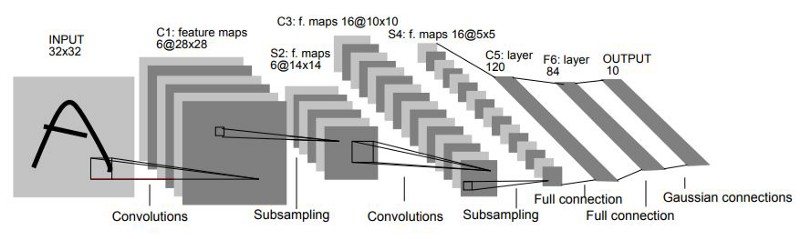
\includegraphics[width=8cm]{../images/cun.jpeg}
  \caption[short]{Architecture of LeNet-5: used for digit recognition and introduced by Yan LeCun \cite{lecun-1998}}
\end{figure}

\subsection{U-Net}
Semantic segmentation, the task of assigning a class label to each pixel in an image, is key to understand an image from a computer vision perspective.
This is the starting point for U-Net which was developed by Ronneberger et al. \cite{ronneberger-2015} to segment images from microscopes in biomedical applications.
U-Net is a fully convolutional architecture that provides accurate and detailed pixel-level predictions.
U-Net is specifically designed to capture both local and global context information.
The U-Net architecture gets its name from its U-shaped design (Figure \ref{fig:unet}), which consists of an encoder path and a decoder path.
The encoder path resembles a traditional CNN and serves the purpose of capturing spatial information
It is made out of multiple convolutional and pooling layers, where each convolutional layer extracts increasingly abstract features by convolving with learnable filters and applying the ReLU activation  .
The decoder path, on the other hand, aims to recover the spatial information lost during the pooling and convolutional operations of the encoder.
It employs a series of transposed convolutional layers to gradually increase the spatial resolution.
The skip connections between the corresponding encoder and decoder layers help preserve fine-grained details that would be otherwise be lost during the encoding process.
UNet is able to segment 2 dimensional images, however in some biomedical contexts 3D scans are used. To segment these kinds of inputs 3D unet was introduced \cite{cicek-2016}.
3D UNet is very similar to 2D UNet except instead of using 2D pooling convolution layers it uses it's 3D counterparts.
We use 3D UNet for our experiments by replacing the depth dimension with our time dimension.

\begin{figure}
  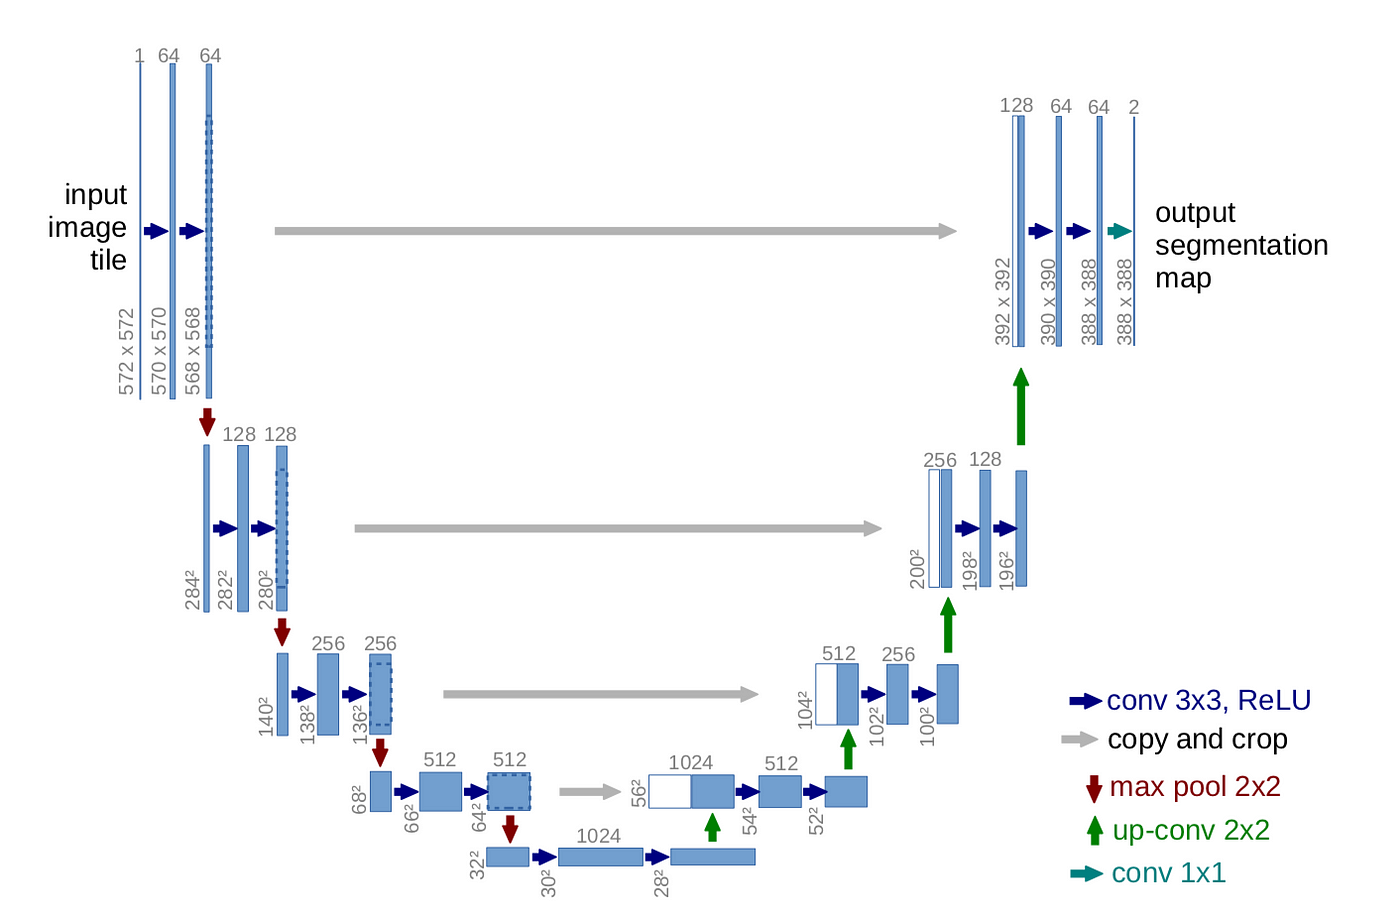
\includegraphics[width=8cm]{../images/unet.png}
  \caption[short]{U-Net}
  \label{fig:unet}
\end{figure}

\subsection{Convolutional LSTM}
The LSTM model, introduced by Hochreiter et al. \cite{lstm}. Solves the issues of gradient explosion and disappearing gradients.
The LSTM model is also more capable of remembering long term dependencies from it's input. This was accomplished by extending the existing RNNs by introducing a long term memory path.
The long term memory path is operated on by the input sequences, the operations that are performed on the long term memory
depend on \textit{gates}. There are two gates that affect the long term memory: the input gate which decides which new information will be added and the forget gate, which decides how much will be forgotten.
LSTM works with vectors, this would be a problem for us because it would mean that we lose some spatial information when we flatten our images. This is why Shi et al. introduced ConvLSTM \cite{convlstm}.
Which replaces the learnable vectors in the LSTM with kernels, and the operations become convolutions.
Here are the equations of the ConvLSTM cell, each ConvLSTM cell produces a short term memory $ \mathcal{H}_{t}$ and a long term memory $\mathcal{C}_{t}$,
the output after passing all of our sequence to the model is the short term memory:

$i_{t} = \sigma\left(W_{xi} * X_{t} + W_{hi} * H_{t-1} + W_{ci} \odot \mathcal{C}_{t-1} + b_{i}\right)$

$f_{t} = \sigma\left(W_{xf} * X_{t} + W_{hf} * H_{t-1} + W_{cf} \odot \mathcal{C}_{-1} + b_{f}\right)$

$\mathcal{C}_{t} = f_{t} \odot \mathcal{C}_{t-1} + i_{t} \odot \text{tanh}\left(W_{xc} * X_{t} + W_{hc} * \mathcal{H}_{t-1} + b_{c}\right)$

$o_{t} = \sigma\left(W_{xo} * X_{t} + W_{ho} * \mathcal{H}_{t-1} + W_{co} \odot \mathcal{C}_{t} + b_{o}\right)$

$ \mathcal{H}_{t} = o_{t} \odot \text{tanh}\left(C_{t}\right) $

\subsection{Attention}
The concept of attention in machine learning comes from the paper by Bahadanau et al \cite{bahdanau-2015}. The authors of
the paper were investigating how to assign different levels of importance to each input in a sequence to sequence model.
Usually attention is computed through a shallow multi-layer perceptron (MLP) since it is expensive to add attention to a model.
However this shallowness is not enough when it comes to computer vision models. Because we are dealing with inputs that are images the amount of connection becomes $(h\times w)^2$
due to the fact that every neuron in the input layer must be connected to the neuron in the output layer.
To address this issue, Axial Attention was introduced by Ho et al. \cite{DBLP:journals/corr/abs-1912-12180} as a means of alleviating this problem.
Axial attention simplifies the computation of attention by exclusively considering the adjacent row and column, thus mitigating the exponential growth of parameters.